%%%%%%%%%%%%%%%%%%%%%%%%%%%%%%%%%%%%%%%%%%%%%%%%%%%%%%%%%%%%%%%%%
%%% %
%%% % Mag.tex
%%% % Praca dyplomowa magisterska
%%% % Krzysztof Lang, 148853
%%% %
%%%%%%%%%%%%%%%%%%%%%%%%%%%%%%%%%%%%%%%%%%%%%%%%%%%%%%%%%%%%%%%%%

\documentclass[12pt,twoside]{article}

\usepackage[section]{placeins}
\usepackage{weiiszablon}

\author{Krzysztof Lang}

% np. EF-123456, EN-654321, ...
\studentID{EF-148853}

\title{Implementacja wybranych algorytmów wypełniania brakujących wartości, dla strumieni dużych zbiorów danych}
\titleEN{Implemetation of selected missing value filling algorithms for large data sets}


%%% wybierz rodzaj pracy wpisując jeden z poniższych numerów: ...
% 1 = inżynierska	% BSc
% 2 = magisterska	% MSc
% 3 = doktorska		% PhD
%%% na miejsce zera w linijce poniżej
\newcommand{\rodzajPracyNo}{2}


%%% promotor
\supervisor{dr Michał Piętal}
%% przykład: dr hab. inż. Józef Nowak, prof. PRz

%%% promotor ze stopniami naukowymi po angielsku
\supervisorEN{Michał Piętal, PhD}

\abstract{Dla poprawnej analizy danych ważna jest ich kompletność.
Istnieje wiele sposobów radzenia sobie z brakującymi danymi.
Najprostsze metody opierające się między innymi na średniej bądź najczęściej występującej wartości w wielu przypadkach
mogą negatywnie wpłynąć na skuteczność analizy. Niniejsza praca ma na celu przeanalizować skuteczność uzupełniania
brakujących danych z użyciem bardziej zaawansowanych metod opierających się na wykorzystaniu uczenia maszynowego.
Te metody mają na celu wypełnić brakujące dane wartościami dużo bardziej zbliżonymi do rzeczywistych,
minimalizując negatywny wpływ na skuteczność późniejszej analizy danych.}
\abstractEN{For correct data analysis, completeness is important. There are many ways to deal with missing data.
The simplest methods based on, among other things, nthe average or the most frequently occurring value
in many cases can negatively affect the effectiveness of the analysis. This paper aims to analyze the effectiveness
of filling in missing data using more advanced methods based on the use of machine learning.
These methods are designed to fill in missing data with values much closer to the actual data,
minimizing the negative impact on the effectiveness of subsequent data analysis.}

\begin{document}

% strona tytułowa
\maketitle

\blankpage

% spis treści
\tableofcontents
\clearpage
\blankpage


\section{Wstęp}

W pierwszym rozdziale przedstawiono zarys treści dalszej pracy.
W drugim rozdziale przybliżono ideę wypełniania brakujących wartości w duzych zbiorach danych,
na co składa się rys historyczny zagadnienia, przedstawienie istniejących rozwiązań i ich znaczenie,
oraz zastanowiono się nad przyszłością zagadnmienia.
Trzeci rozdział przybliża narzędzia użyte do przygotowania części praktycznej niniejszej pracy,
to jest programu realizującego testy algorytmów wypełniajacych puste miejsca oraz
dane wykorzystane do testów.
Na rodział czwarty składa się opis praktycznej części badań. 
Znajduje się w nim opis przygotowanego programu wraz z przykłądem działana, opisy zaimplementowanych algorytmów,
oraz przedstawione zostały wyniki przeprowadzonych testów.
Rozdział piąty składa się z podsumowania przeprowadzonych działań i przedstawienia wyciągniętych wniosków.

\clearpage


\section{Wprowadzenie do wypełniania brakujących wartości}

\subsection{Rys historyczny}
\subsection{Na czym polega wypełnianie brakujących wartości}
\subsection{Korzyści i zagrożenia}
\subsection{Perspektywy na przyszłość}
\clearpage


\section{Omówienie narzędzi i danych}

\subsection{Python}

Python to interpretowany język wysokiego poziomu o ogólnym zastosowaniu.
Stworzony został w roku 1991 przez Guido van Rossum i jest wciąż wciąż rozwijany.
Najnowsza stabilna wersja to 3.11.2.

Python znany jest ze swojej prostej do zrozumienia składni,
czytelnego kodu, wsparcia różnych paradygmatów programowania (obiektowego, imperatywnego, funkcyjnego),
dużej biblioteki standardowej i bardzo szerokiego wyboru dodatkowych bibliotek. \cite{python}

Do słabszych stron języka zaliczyć można słabą wydajność pod względem prędkości działania i wykorzystania pamięci
bądź problemy z kompatybilnością kodu napisanego w różnych wersjach lub implementacjach Pythona.

\subsection{Visual Studio Code}

Jako środowisko programowania wybrano "Microsoft Visual Studio Code".
Jest to darmowy edytor kodu o otawrtym kodzie. Stworzony został przez firmę Microsoft w roku 2015.
Zaprojektowany został z myślą tworzenia nowoczesnych aplikacji webowych i chmurowych z wykorzystaniem wielu języków. \cite{VSC}
Ze wzglądu na otwartość kodu, dostępne jest wiele rozszerzeń do programu,
które znacznie ułatwiają tworzenie nawet skomplikowanych projektów.

W celu umożliwienia pracy nad programem z wielu urządzeń
oraz dla zachowania pełnej historii tworzenia programu wykorzystano integrację "Visual Studio Code" z repozytorium GitHub.
\subsection{Biblioteki}
\subsubsection{Pandas}

Pandas to popularna biblioteka służąca manipulacji i analizy danych w Pythonie.
Stworzona została w roku 2008 przez Wesa McKinney i jest stale rozwijana przez dużą grupę deweloperów.
Nazwa Pandas pochodzi od "Python data analysis".
Najważniejsze zalety Pandas to:

\begin{itemize}[label=-,labelsep=0.4cm, leftmargin=1.25cm]
    \item wsparcie dla wielu formatów danych, w tym CSV, Excel, SQL i inne,
    \item duża szybkość przeprowadzania operacji na danych,
    \item obsługa brakujących wartości w danych,
    \item łatwa integracja z innymi popularnymi bibliotekami,
    \item bardzo rozbudowana dokumentacja.
\end{itemize}

Pandas wykorzystuje dwie główne struktury danych: "Series" i "DataFrame".
Ta pierwsza to jednowymiarowa tablica wartości posiadająca indeksy każdego elementu,
z kolei druga to dwuwymiarowa tablica wartości z indeksami zarówno rzędów jak i kolumn.
Obydwie struktury mogą przechowywać dowolne typy danych. \cite{pandas}

\subsubsection{NumPy}

NumPy to biblioteka dla Pythona wykorzystywana do pracy na obiektach będących wielowymiarowymi tablicami
oraz udostęniajaca szereg narzędzi do obliczeń naukowych. Została stworzona w roku 2005 przez Travisa Oliphant
jako następca bibliotek Numeric \cite{numeric} i Numarray \cite{numarray}. Biblioteka jest wciąż rozwijana przez zaangażowaną grupę programistów.
NumPy jest szeroko wykorzystywana do przeprowadzania obliczeń naukowych ze względu na szereg zalet:

\begin{itemize}[label=-,labelsep=0.4cm, leftmargin=1.25cm]
    \item wspiera wielowymiarowe tabele, zarówno o homogenicznych jak i heterogenicznych typach danych,
    \item oferuje dużą ilość funkcji matematycznych, generatorów liczb pseudolosowych, transformat i innych narzędzi
    przydatnych w zastosowaniach naukowych,
    \item łatwo integruje się z innymi bibliotekami,
    \item posiada bardzo rozbudowaną dokumentację.
\end{itemize}

Do wad zaliczają się stosunkowo niska wydajność i problemy z obsługą niektórych typów danych i brakujących wartości. \cite{numpy}

\subsubsection{SciEKit-learn}

SciKit-learn to biblioteka zawierająca narzędzia związane z uczeniem maszynowym dla Pythona.
Jest częścią większego zestawu narzędzi SciKit,
zawierającego biblioteki oferujące szeroki wachlarz narzędzi do analizy danych.
Początkowo stworzony przez Davida Cournapeau jako projekt w ramach "Google Summer of Code" w roku 2007,
został później przepisany i rozwinięty głównie przez Francuski Instytut Badań w Dziedzinie Informatyki i Automatyki (INRIA)
i udostępniony publicznie w roku 2010.
SciKit-learn przestrzega zasad projektowania API dla oprogramowania uczenia maszynowego,
które obejmują między innymi spójność, rozsądne domyślne ustawienia i dokumentację. \cite{scikit}

\subsubsection{EasyGUI}

EasyGUI to biblioteka Pythona służaca do implementacji prostego interfejsu graficznego.
Został stworzony przez Stephena Ferg i udostęniony w roku 2004. Oparty jest na bibliotece Tkinter \cite{tkinter}.
Główną zaletą EasyGUI jest jego prosta składnia, pozwalajaca na tworzenie nieskomplikowanych aplikacji bez
konieczności uczenia się stosowania bardziej zaawansowanych bibliotek.
Osiągnięte to zostało przez zastosowanie predefiniowanych okien spełniających najczęściej wykorzystywane role,
taklie jak okna wyboru, wyświetlanie wiadomości, wpisywanie tekstu i inne.
Niestety zaprzestano dalszego rozwoju biblioteki, przez co nie można spodziewać się dodania nowych funkcji
czy popraw działania istniejących. \cite{easygui}

\subsection{Źródła danych}

\subsubsection{Użyte repozytoria danych}

Aby wyniki badań niosły ze sobą odpowiednią wartość merytoryczną,
potrzebne są odpowiednie zbiory danych na których zostaną przeprowadzone testy.
W celu znalezienia odpowiednich zbiorów danych, przyjęto następujące założenia:

\begin{itemize}[label=-,labelsep=0.4cm, leftmargin=1.25cm]
    \item zbiór danych musi być wystarczająco duży,
    \item zbiór danych musi zawierać odpowiedniż ilość atrybutów aby modele decyzyjne miały
    do dyspozycji wystarczającą ilość danych uczących,
    \item atrybuty powinny zawierać różnorodne typy danych w celu przetestowania wypełniania zarówno danych
    liczbowych (całkowitych i zmiennoprzecinkowych) jak i kategorycznych,
    \item zbiór danych nie może mieć pustych wartości.
\end{itemize}

Do wyszukania odpowiednich zbiorów danych wykorzystano narzędzie "Google Dataset Search".
Z jego pomocą wybrano 2 zbiory danych z róźnych dziedzin.
Po uprzedniej ich obróbce zostały wykorzystane do przeprowadzenia testów algorytów wypełniania.
\subsubsection{Adult Data Set}

Zbiór danych "Adult Data Set" zawiera dane ze spisu ludności przeprowadzonego w roku 1994 w Stanach Zjednoczonych.
Jest szeroko wykorzystywany do testowania uczenia maszynowego.
Zawiera ponad 30000 rekordów i 15 atrybutów. \cite{adult} Opis atrybutów:
\begin{itemize}[label=-,labelsep=0.4cm, leftmargin=1.25cm]
    \item age: wiek spisanej osoby, liczba całkowita,
    \item workclass: rodzaj zatrudnienia, dane kategoryczne, 8 możliwych wartości,
    \item fnlwgt: jaka proporcja populacji ma identyczny zestaw pozostałych wartości, liczba całkowita,
    \item education: osiągnięty poziom edukacji, dane kategoryczne, 16 możliwych wartości,
    \item education-num: osiągnięty poziom edukacji zakodowany jako liczba całkowita,
    \item martial-status: status matrymonialny, dane kategoryczne, 7 możliwych wartości,
    \item occupation: zawód, dane kategoryczne, 14 możliwych wartości,
    \item relationship: rola w związku, dane kategoryczne, 6 możliwych wartości,
    \item race: klasyfikacja rasowa, dane kategoryczne, 5 możliwych wartości,
    \item sex: płeć, dane kategoryczne, 2 możliwe wartości,
    \item capital-gain: zysk kapitału w zwiazku z inwestycjami, liczba całkowita,
    \item capital-gain: strata kapitału w zwiazku z inwestycjami, liczba całkowita,
    \item hours-per-week: ilość godzin pracujących w tygodniu, liczba całkowita,
    \item native-country: kraj pochodzenia, dane kategoryczne, 41 możliwych wartości,
    \item attribute: czy osoba zarabia powyżej czy poniżej 50000\$ rocznie.
\end{itemize}
Ten zbiór danych został wybrany ze względu na występowanie zarówno atrybutów liczbowych jak i kategorycznych,
zadowalajacą ilość rekordów oraz atrybutów.
Ma na celu przetestowanie skuteczności działania algorytmów do wypełniania brakujących miejsc
w zbiorach danych z brakami w danych o różnych typach.
Nie wymaga dodatkowej obróbki przed rozpoczęciem testów. 
\subsubsection{Stock Exchange Data}

Zbiór danych "Stock Exchange Data" zawiera informacje o cenach akcji na giełdach w różnych krajach w latach 1965-2021.
Dane zostały zebrane z "Yahoo Finance", posiadającego dane o giełdzie z wielu lat w wielu krajach.
Posiada ponad 100000 rekordów i 9 atrybutów. \cite{stock} Opis atrybutów:
\begin{itemize}[label=-,labelsep=0.4cm, leftmargin=1.25cm]
    \item Index: symbol wskazujacy z jakiej giełdy pochodzą dane, dane kategoryczne, 5 możliwych wartości,
    \item Date: data obserwacji, dane kategoryczne,
    \item Open: cena akcji podczas otwarcia, liczba wymierna,
    \item High: najwyższa cena w ciągu dnia, liczba wymierna,
    \item Low: najniższa cena w ciągu dnia, liczba wymierna,
    \item Close: cena akcji w momencie zamknięcia, liczba wymierna,
    \item Adj Close: cena akcji w momencie zamknięcia skorygowana o podziały jak i dywidendy, liczba wymierna,
    \item Volume: liczba akcji będących przedmiotem obrotu w ciągu dnia sesyjnego, liczba całkowita,
    \item CloseUSD: cana akcji w momencie zamknięcia wyrażona w dolarach amerykańskich
\end{itemize}
Ten zbiór danych został wybrany ze względu na bardzo popularną kategorię danych, to jest dane finansowe.
Ma na celu przetestowanie skuteczności działania algorytmów w przypadku danych numerycznych,
w szególności liczb wymiernych.
W celu lepszego przygotowania do testów zakodowano kolumnę "Data" z wykorzystaniem "label encoding",
to jest zamiany danych na postać numeryczną.
Usunięto też rekordy posiadające wartość "0" w kolumnie "Volume".
Ich duża ilość (ponad 30\%) mogła by negatywnie wpłynąć na uczenie modeli decyzyjnych.
W wyniku tego zmniejszono liczbę rekordów do ponad 62000,
co wciąż jest ilością spełniajacą założenia dla zbiorów danych.


\clearpage
\section{Implementacja i testy}
\subsection{Opis przygotowanego programu}
\subsubsection{Założenia i realizacja}
Założono, że program ma rtealizować 3 zadania:

\begin{enumerate}[label=\arabic*), leftmargin=1.25cm]
    \item Przygotować dane do wypełniania poprzez sztuczne utworzenie brakujacych wartości.
    \item Wypełnić brakujące wartości z wykorzystaniem wybranych algorytmów.
    \item Ocenić skuteczność wypełniania w celu porównania algorytmów.
\end{enumerate}

Poszczególne zadania zrealizowano jako osobne moduły.

Przyjęto też następujące założenia:

\begin{enumerate}[label=\arabic*), leftmargin=1.25cm]
    \item Wykorzystanym językiem ma być Python.
    \item Program ma być napisany zgodnie z paradygmatem programowania obiektowego.
    \item Poszczególne klasy mają być zawarte w osobnych plikach.
    \item Interakcja z programem ma opierać się o prosty interfejs graficzny.
    \item Dostęp do wszystkich modułów programu ma być zapewniony z jednego miejsca.
    \item Pliki wygenerowane przez jeden moduł mają być przygotowane w sposób umożliwiający
    wykorzystanie ich przez kolejny. Oprócz odpowiedniego formatowania wewnątrz pliku,
    oznacza to przyjęcie konwencji nazewnictwa plików opartej o prefiksy i sufiksy.
\end{enumerate}

Program składa się z następujacych plików:

\begin{itemize}[label=-,labelsep=0.4cm, leftmargin=1.25cm]
    \item mgr\_main.py: główny plik nie zawierający żadnej klasy, odpowiadający za wybór modułu do uruchomienia,
    i uruchomienie odpowiedniego modułu po wybraniu,
    \item mgr\_nan\_gen" plik zawierajacy klasę "NanGen", odpowiadającą za realizację modułu przygotowujacego plik,
    \item mgr\_fill.py: plik zawierający klasę "Fill", odpowiadającą za realizację modułu wypełniajacego brakuące dane,
    \item mgr\_data.py: plik zawierający klasę "Data",
    odpowiadającą za wybranie pliku do wypełnienia i przygotowanie do do dalszej obróbki, oraz klasę "PrepareData",
    odpowiadającą za przygotowanie danych do przekazania silnikowi uczenia maszynowego celem wypełnienia
    oraz późniejszemu przywróceniu danym ich pierwotnego wyglądu
    \item mgr\_di.py: plik zawierjący klasę DownImpu,
    odpowiadającą za przygotowanie danych dla algorytmu "Downward Imputation"
    \item mgr\_temp\_fill: plik zawierający klasę "TempFill", odpowiadającą za tymczasowe wypełnianie brakujących miejsc,
    potrzebne podczas przygotowywania danych dla algorytmu "Prostego"
    \item mgr\_acc: plik zawierający klasę "AccuracyTester", odpowiadającą za obliczanie skuteczności wypełniania danych
\end{itemize}

Wykorzystując narzędzie "auto-py-to-exe", utworzono plik "mgr\_suite.exe",
pozwalajacy uruchomić program bez konieczności instalowania interpretera Python i potrzebnych bibliotek. \cite{autopy}

\subsubsection{Działanie programu}
Poniżej zaprezentowano działanie programu na przykładzie pliku data\_stock.csv.
Zostanie on najpierw przygotowany do testów,
następnie brakujace dane zostaną wypełnione z wykorzystaniem jednego z algorytmów,
po czym zostanie obliczona dokładność tego wypełnienia.

% Uruchomienie
Po uruchomieniu "mgr\_suite.exe" wyświetlone zostaje okno służące do wyboru modułu, pokazane na rysunku \ref{Fig:main}.

\begin{figure}[ht]
	\centering
	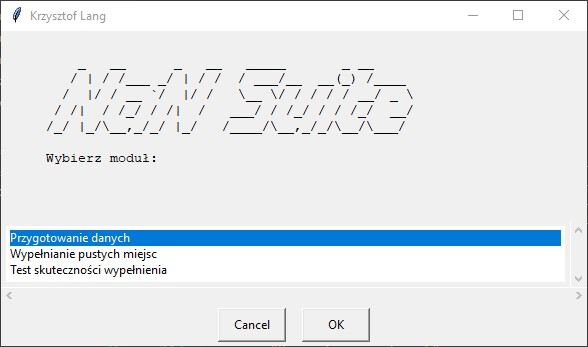
\includegraphics[width=12cm]{img/01.jpg}
	\caption{Główne okno programu, pozwalajace na wybór modułu do uruchomienia}
\label{Fig:main}
\end{figure}
\FloatBarrier
% Przygotowanie danych

Pierwszy moduł odpowiada za przygotowanie danych do wypełniania poprzez usunięcie losowych wartości ze zbioru danych.
Pierwszym krokiem jest wybranie pliku który ma zostać przygotowany
z użyciem okna pokazanego na rysunku \ref{Fig:gen_file}.
Lista plików generowana jest na podstawie plików znajdujących się
w tym samym folderze co uruchamiany program spełniających założony format nazwy.
Założono, że pliki które nadają się do wypełnienia mają być zapisane w formacie CSV,
natomiast nazwa zaczynać się ma od prefiksu "data\_" i nie posiadać żadnych sufiksów.

\begin{figure}[ht]
	\centering
	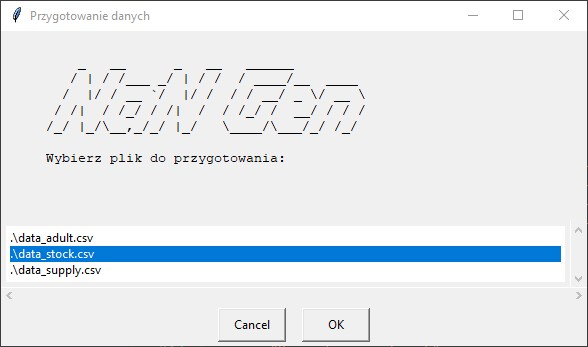
\includegraphics[width=12cm]{img/02.jpg}
	\caption{Okno wyboru pliku do przygotowania}
\label{Fig:gen_file}
\end{figure}
\FloatBarrier

Następnie wybrane z listy zostają kolumny w których maja zostać usunięte dane.
Wyboru dokonuje się z użyciem okna pokazanego na rysunku \ref{Fig:gen_col}.
Kolumny do wyboru zaczerpnięte są bezpośrednio z załadowanego wcześniej pliku.
Wybrać można dowolną ilość, lecz zalecane jest poniżej 50\%.

\begin{figure}[ht]
	\centering
	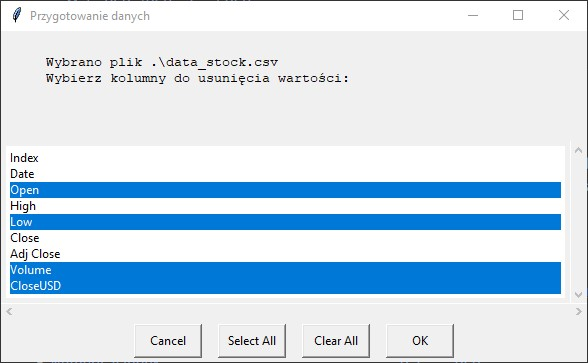
\includegraphics[width=12cm]{img/03.jpg}
	\caption{Okno wyboru kolumn}
\label{Fig:gen_col}
\end{figure}
\FloatBarrier

W wybranych kolumnach zostaje usunięte od 5\%
do 15\% wartości - dla każdej kolumny ilość jest losowana.
Dodatkowo stworzony zostaje plik przechowujęcy informacje które wartości zostały usunięte.
Ta informacja zostaje później wykorzystana do oceny skuteczności wypełnienia zbioru danych.
Po zakończeniu usuwania wartości wyświetlone zostaje okno z podsumowaniem jak na rysunku \ref{Fig:gen_end}.
Nazwa utworzonego pliku z gotowymi danymi tworzona jest
poprzez dodanie sufiksu "\_holes\_X" do nazwy oryginalnego pliku, gdzie X to kolejna liczba naturalna.
Umożliwia to tworzenie plików z danymi usuniętymi z różnych zestawów kolumn bez konieczności ręcznej zmiany ich nazw.
Nazwa pliku z informacją które dane zostały usunięte tworzona jest
przez dodanie sufiksu "\_journal" do nazwy oryginalnego pliku.

\begin{figure}[ht]
	\centering
	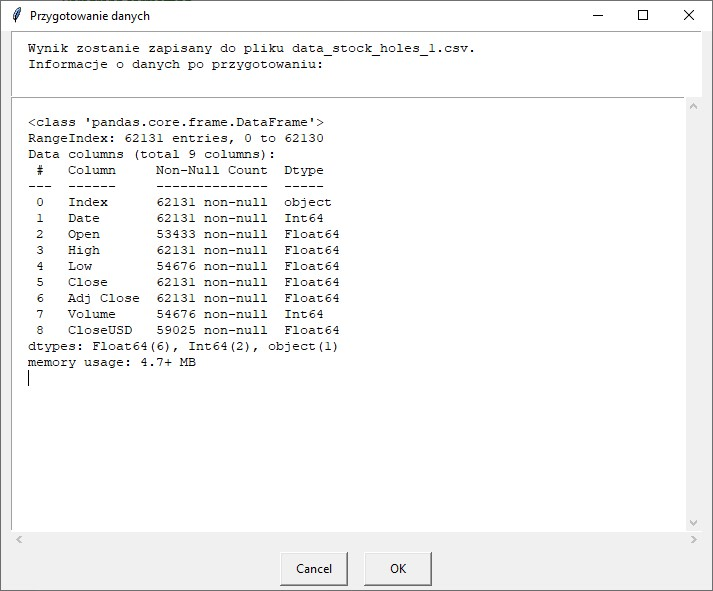
\includegraphics[width=12cm]{img/04.jpg}
	\caption{Okno z podsumowaniem}
\label{Fig:gen_end}
\end{figure}
\FloatBarrier

% Wypełnianie brakujących wartości

Drugi moduł służy do wypełniania brakujacych wartości w zbiorze danych z użyciem wybranego algorytmu. 

Najpierw należy wskazać plik który ma zostać wypełniony z użyciem okna wyboru pokazanego na rysunku \ref{Fig:fill_file}.
Tak jak wcześniej, lista tworzona jest na podstawie plików w folderze i przyjętej konwencji nazewnictwa plików.
Wyświetlane są wyłącznie pliki posiadające sufiks "\_holes\_X" w nazwie, bez kolejnych sufiksów.

\begin{figure}[ht]
	\centering
	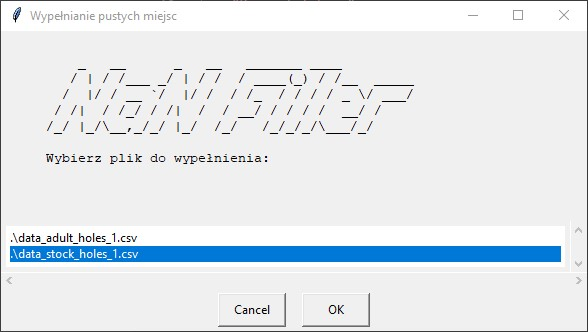
\includegraphics[width=12cm]{img/05.jpg}
	\caption{Okno wyboru pliku do wypełnienia}
\label{Fig:fill_file}
\end{figure}
\FloatBarrier

Następnie z użyciem okna jak na rysunku \ref{Fig:fill_alg}
wybrany zostaje algorytm który ma zostać wykorzystany do wypełniania brakujących wartości.
Wyświetlona zostaje też nazwa wybranego wcześniej pliku w celu uniknięcia błędu wybrania niewłaściwego pliku.

\begin{figure}[ht]
	\centering
	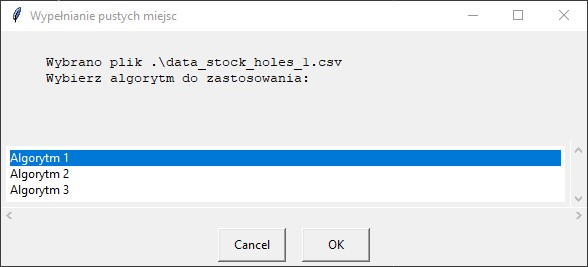
\includegraphics[width=12cm]{img/06.jpg}
	\caption{Okno wyboru algorytmu}
\label{Fig:fill_alg}
\end{figure}
\FloatBarrier

Puste miejsca zostają wypełnione z wykorzystaniem wybranego algorytmu.
Dokładny sposób działania algorytmów zostanie opisany w kolejnych rozdziałach.
Po zakończeniu wypełniania wyświetlone zostaje podsumowanie jak na rysunku \ref{Fig:fill_end}.
Nazwa pliku wynikowego tworzona jest poprzez dodanie sufixu "\_filled\_Y", gdzie Y to nazwa wybranego algorytmu.

\begin{figure}[ht]
	\centering
	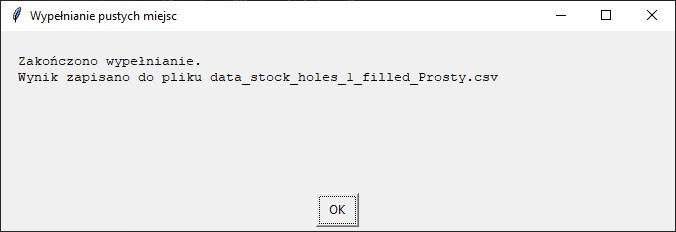
\includegraphics[width=12cm]{img/07.jpg}
	\caption{Okno z podsumowaniem wypełniania}
\label{Fig:fill_end}
\end{figure}
\FloatBarrier

% Sprawdzenie skuteczności wypełniania

Ostatni moduł odpowiada za wygenerowanie danych,
które można wykorzystać do oceny skuteczności wypełniania brakujących wartości.
Jako wystarczające uznano procent skuteczności wypełniania dla danych kategorycznych i liczb całkowitych
oraz średnie odchylenie bezwzględne dla wszystkich danych liczbowych.
Obie wartości są obliczane dla poszczególnych wypełnionych kolumn.

Jak w przypadku poprzednich modułów, zacząć należy od wyboru pliku który ma zostać poddany analizie.
Wyboru dokonuje się z użyciem okna pokazanego na rysunku \ref{Fig:acc_file}.
Wyświetlane są tylko pliki zawierające słowo "filled" w nazwie, ponieważ takie pliki
posiadają wartości wypełnione za pomocą któregoś algorytmu z użyciem odpowiedniego modułu.

\begin{figure}[ht]
	\centering
	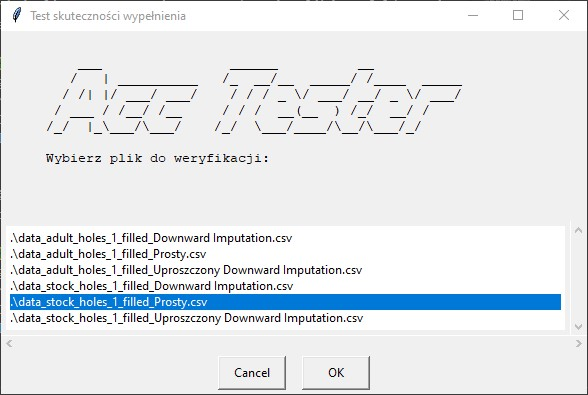
\includegraphics[width=12cm]{img/08.jpg}
	\caption{Okno wyboru pliku do analizy}
\label{Fig:acc_file}
\end{figure}
\FloatBarrier

Z użyciem wybranego pliku, oryginalnego pliku z danymi przed usunięciem losowych danych
oraz pliku z informacją które dane zostały usunięte a następnie wypełnione,
przeprowadzane jest obliczanie skuteczności wypełniania danych.

Obliczenie procentowej skuteczności wypełnienia przebiega następująco:

\begin{enumerate}[label=\arabic*), leftmargin=1.25cm]
    \item Sprawdzenie ilości wypełnianych wartości w danej kolumnie.
    \item Zsumowanie ilości poprawnie wypełnionych danych w kolumnie poprzez porównanie wartości o współrzędnych
    zapisanych w pliku tworzonym podczas przygotowywania danych.
    \item Zastosować wzór \ref{Eq:acc}:
        \begin{equation}
        ACC=\frac{m}{n}\times100\%
        \label{Eq:acc}
        \end{equation}
    gdzie: $ACC$ -- procentowa skuteczność wypełnienia kolumny,
    $m$ -- ilość poprawnie wypełnionych wartości,
    $n$ -- ilość wypełnionych wartości.
\end{enumerate}

Aby obliczyć średnie odchylenie bezwzględne należy zastosować wzór \ref{Eq:aad}:

    \begin{equation}
    AAD=\frac{\sum_{i=1}^{n}|x_i - \hat{x_i}|}{n}
    \label{Eq:aad}
    \end{equation}

gdzie: $AAD$ -- średnie odchylenie bezwzględne dla danej kolumny,
$n$ -- ilość wypełnionych wartości w kolumnie,
$x_i$ -- wartość wypełnionego $i$-tego elementu kolumny,
$\hat{x_i}$ -- oryginalna wartość $i$-tego elementu kolumny.

Po zakończeniu obliczeń, wyświetlane jest podsumowanie jak na rysunku \ref{Fig:acc_end},
a wynik obliczeń zapisywany jest w dwóch plikach

\begin{itemize}[label=-,labelsep=0.4cm, leftmargin=1.25cm]
    \item wyniki obliczania procentowej skuteczności jest zapisywany w pliku o nazwie
    tworzonej przez dodanie do nazwy analizowanego pliku sufiksu "\_aad",
    \item wyniki obliczania średniego odchylenia bezwzględnego jest zapisywany w pliku o nazwie
    tworzonej przez dodanie do nazwy analizowanego pliku sufiksu "\_acc".
\end{itemize}

\begin{figure}[ht]
	\centering
	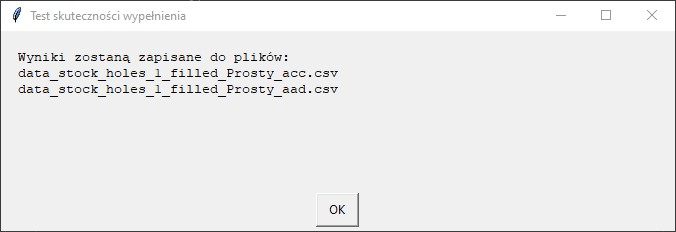
\includegraphics[width=12cm]{img/09.jpg}
	\caption{Okno z podsumowaniem}
\label{Fig:acc_end}
\end{figure}
\FloatBarrier

\subsection{Opis implementacji algorytmów}

Implementowane algorytmy opierają się o kolejne rozwinięcia idei zaprezentowanej przez Piętal M. w \cite{wyb_zag}.
Polega ona na sformułowaniu problemu wypełniania problemu wypełniania brakujących wartości jako problemu decyzyjnego.
Wynikają z tego następujące założenia:
\begin{itemize}[label=-,labelsep=0.4cm, leftmargin=1.25cm]
    \item kolumny wypełniane są pojedyńczo,
    \item samo wypełnianie przeprowadzane jest przez system decycyjny,
    \item algorytm ma za zadanie wybrać kolejność wypełniania kolumn oraz
    określić jakie kolumny będą zawarte w zbiorze danych uczących systemu decyzyjnego.
\end{itemize}

Działanie poszczególnych algorytmów zostanie zaprezentowane na przykładowej tabeli \ref{tab:base}
przedstawiającej zbiór danych:
\begin{table}[ht]
\caption{Tabela wyjściowa}
\centering
    \begin{tabular}{|c|c|c|c|c|c|c|c|c|c|c|c|c|c|c|}
        \hline
           & A & B & C & D & E & F & G & H & I & J & K & L & M & N \\ \hline
        1  & * & * & x & * & * & * & x & * & * & * & x & * & * & * \\ \hline
        2  & x & * & * & * & * & * & * & * & * & * & * & x & * & * \\ \hline
        3  & * & * & * & * & x & * & * & * & * & * & * & x & * & * \\ \hline
        4  & x & * & x & * & x & * & x & x & * & * & x & x & * & * \\ \hline
        5  & * & * & * & * & x & * & * & x & x & * & * & * & * & * \\ \hline
        6  & * & * & * & * & x & * & x & x & * & * & * & * & * & * \\ \hline
        7  & * & * & * & * & x & * & * & * & * & * & * & * & * & * \\ \hline
        8  & * & * & * & * & * & * & * & x & * & * & x & * & x & * \\ \hline
        9  & * & * & * & * & x & * & * & * & x & * & * & * & x & * \\ \hline
        10 & * & * & * & * & * & * & x & * & x & * & * & * & * & * \\ \hline
        11 & * & x & * & * & x & * & * & * & * & * & * & * & * & * \\ \hline
    \end{tabular}
\label{tab:base}
\end{table}
\FloatBarrier
gdzie: $*$ -- istniejąca wartość, $x$ -- brakująca wartość.

\subsubsection{Prosty}

Procedura dla algorytmu prostego wygląda następująco:

\begin{enumerate}[label=\arabic*), leftmargin=1.25cm]
    \item Tworzony jest zbiór kolumn z brakującymi wartościami $X$.
    Dla przykładowej tabeli będzie to zbiór $X=\{A,B,C,E,G,H,I,K,L,M\}$.
    \item Kolumny w zbiorze $X$ są następnie sortowane od kolumn zawierających
    najmniejszą ilość brakujących wartości do zawierających ich najwięcej, dając ciąg $\eta$.
    W przypadku kolumn o takiej samej ilości brakujących danych kolejność nie ma znaczenia.
    Dla przykładowej tabeli zbiór ten będzie wyglądał następująco: $\eta=(B,M,C,A,L,K,I,H,G,E)$.
    \item Pierwszy element w ciągu $\eta$ zostaje wybrany jako kolumna która zostanie wypełniona.
    W przykładzie będzie to element $B$.
    \item Tabela zostaje rozdzielona na dwie: w jednej znajdują się rekordy
    w których w kolumnie wybranej do wypełnienia znajdują się dane,
    a w drugiej rekordy w których w wybranej tabeli danych brakuje.
    Dla przykładowej tabeli będzie to wyglądało następująco,
    gdzie tabela \ref{tab:simple_full} przedstawia tabelę z danymi w wybranej kolumnie,
    natomiast tabela \ref{tab:simple_nan} przedstawia tabelę z brakiem danych w wybranej kolumnie.
    Dla lepszej czytelności, przesunięto rozważaną kolumnę na początek tabeli:

        \begin{table}[ht]
        \caption{Tabela wydzielona z oryginalnej, zawierająca wyłacznie rekordy z danymi w rozważanej kolumnie}
        \centering
            \begin{tabular}{|c|c|c|c|c|c|c|c|c|c|c|c|c|c|c|}
                \hline
                   & A & B & C & D & E & F & G & H & I & J & K & L & M & N \\ \hline
                1  & * & * & x & * & * & * & x & * & * & * & x & * & * & * \\ \hline
                2  & x & * & * & * & * & * & * & * & * & * & * & x & * & * \\ \hline
                3  & * & * & * & * & x & * & * & * & * & * & * & x & * & * \\ \hline
                4  & x & * & x & * & x & * & x & x & * & * & x & x & * & * \\ \hline
                5  & * & * & * & * & x & * & * & x & x & * & * & * & * & * \\ \hline
                6  & * & * & * & * & x & * & x & x & * & * & * & * & * & * \\ \hline
                7  & * & * & * & * & x & * & * & * & * & * & * & * & * & * \\ \hline
                8  & * & * & * & * & * & * & * & x & * & * & x & * & x & * \\ \hline
                9  & * & * & * & * & x & * & * & * & x & * & * & * & x & * \\ \hline
                10 & * & * & * & * & * & * & x & * & x & * & * & * & * & * \\ \hline
            \end{tabular}
        \label{tab:simple_full}
        \end{table}
        \FloatBarrier

        \begin{table}[ht]
        \caption{Tabela wydzielona z oryginalnej, zawierająca wyłacznie rekordy z brakiem danych w rozważanej kolumnie}
        \centering
            \begin{tabular}{|c|c|c|c|c|c|c|c|c|c|c|c|c|c|c|}
                \hline
                   & A & B & C & D & E & F & G & H & I & J & K & L & M & N \\ \hline
                11 & * & x & * & * & x & * & * & * & * & * & * & * & * & * \\ \hline
            \end{tabular}
        \label{tab:simple_nan}
        \end{table}
        \FloatBarrier

    \item Pierwsza z tabel - w przykładzie tabela \ref{tab:simple_full} - posłuży do uczenia modelu uczenia maszynowego.
    Wypełniana kolumna służy jako cel, a pozostałe jako dane uczące.
    \item Następnie nauczony model zostaje wykorzystany do wypełnienia brakujących wartości w drugiej tabeli,
    w przykładzie tabeli \ref{tab:simple_nan}.
    \item Na koniec tabele są łączone w jedną co w przykładzie poskutkuje tabelą \ref{tab:simple_end},
    a algorytm jest powtarzany aż do wypełnienia wszystkich brakujących wartości.

    \begin{table}[ht]
        \caption{Tabela prezentująca wygląd danych po pojedynczym przejściu algorytmu}
        \centering
            \begin{tabular}{|c|c|c|c|c|c|c|c|c|c|c|c|c|c|c|}
                \hline
                   & A & B & C & D & E & F & G & H & I & J & K & L & M & N \\ \hline
                1  & * & * & x & * & * & * & x & * & * & * & x & * & * & * \\ \hline
                2  & x & * & * & * & * & * & * & * & * & * & * & x & * & * \\ \hline
                3  & * & * & * & * & x & * & * & * & * & * & * & x & * & * \\ \hline
                4  & x & * & x & * & x & * & x & x & * & * & x & x & * & * \\ \hline
                5  & * & * & * & * & x & * & * & x & x & * & * & * & * & * \\ \hline
                6  & * & * & * & * & x & * & x & x & * & * & * & * & * & * \\ \hline
                7  & * & * & * & * & x & * & * & * & * & * & * & * & * & * \\ \hline
                8  & * & * & * & * & * & * & * & x & * & * & x & * & x & * \\ \hline
                9  & * & * & * & * & x & * & * & * & x & * & * & * & x & * \\ \hline
                10 & * & * & * & * & * & * & x & * & x & * & * & * & * & * \\ \hline
                11 & * & * & * & * & x & * & * & * & * & * & * & * & * & * \\ \hline
            \end{tabular}
        \label{tab:simple_end}
        \end{table}
        \FloatBarrier
\end{enumerate}

\subsubsection{Uproszczony Downward Imputation}
\subsubsection{Downward Imputation}
\subsection{Napotkane problemy}
\subsection{Testy algorytmów na wybranych źródłach danych}
\clearpage


\section{Podsumowanie i wnioski końcowe}

\clearpage


\section*{Załączniki}

\addcontentsline{toc}{section}{Załączniki}

\clearpage


\addcontentsline{toc}{section}{Literatura}

\begin{thebibliography}{4}
    % Narzędzia
    \bibitem{python} https://www.python.org/. Dostęp 26.02.2023.
    \bibitem{VSC} https://code.visualstudio.com/. Dostęp 26.02.2023.
    % Biblioteki
    \bibitem{pandas} https://pandas.pydata.org/. Dostęp 26.02.2023.
    \bibitem{numeric} https://pypi.org/project/Numeric/. Dostęp 26.02.2023.
    \bibitem{numarray} https://pypi.org/project/numarray/. Dostęp 26.02.2023.
    \bibitem{numpy} https://numpy.org/. Dostęp 26.02.2023.
    \bibitem{scikit} https://scikit-learn.org/stable/. Dostęp 26.02.2023.
    \bibitem{tkinter} https://docs.python.org/3/library/tkinter.html. Dostęp 26.02.2023.
    \bibitem{easygui} https://easygui.sourceforge.net/. Dostęp 26.02.2023.
    % Źródła danych
    \bibitem{adult} https://archive-beta.ics.uci.edu/dataset/2/adult. Dostęp 26.02.2023.
    \bibitem{stock} www.kaggle.com/datasets/mattiuzc/stock-exchange-data. Dostęp 26.02.2023.
    \bibitem{autopy} https://pypi.org/project/auto-py-to-exe/. Dostęp 26.02.2023.
    % Implementacja
    \bibitem{wyb_zag} Brański A.: Wybrane zagadnienia informatyki stosowanej. Oficyna Wydawnicza Politechniki Rzeszowskiej, Rzeszów 2020.
\end{thebibliography}

\clearpage


\makesummary

\end{document} 
